\documentclass{fisatproject}
\title{Hologram with Haptic Feedback}
\team{Leo Varghese \\ Mohit Rajan E\\ Riya Alexander}
\author{Mohit Rajan E}
\begin{document}
\maketitle
\makecert

\newpage
\pagenumbering{roman}
\setcounter{page}{1}
\newgeometry{top=4cm,bottom=0.1cm}
\thispagestyle{plain}
\renewcommand\abstractname{ABSTRACT}
\begin{abstract}
\vspace{5cm}
This paper is intended to analyze and discuss the developments made so far in the field of holography and holographic projection, it discusses the doability and the eventuality in the field of touchable holograms, which works in gear with hand gestures. In this paper, first some elementary matters about what a hologram is and a concise description of how they are devised is discussed. Then how hologram interact with our hand gestures and provide haptic feedback is discussed. In this paper the focus is on the feasibility or doability study of some methods and the analysis and consequences of these methods. Challenges in the whole process will be confronted and then some discussion about future scopes of this technology and where this technology can lead us is done.
\end{abstract}



\newpage
\renewcommand\abstractname{Contribution by Author}
\thispagestyle{plain}
\begin{abstract}
\vspace{5cm}
Author Contribution  Goes Here
\vspace{1cm}
\begin{flushright}
Student Name
\end{flushright}
\end{abstract}

\newpage
\renewcommand\abstractname{ACKNOWLEDGMENT}
\thispagestyle{plain}
\begin{abstract}
\vspace{5cm}
Your Acknowledgement Goes Here
\vspace{1cm}
\begin{flushright}
Student 1
\end{flushright}
\end{abstract}
\newpage

\restoregeometry
\tableofcontents
\newpage

\cleardoublepage
\addcontentsline{toc}{chapter}{\listfigurename}
\listoffigures
\newpage

\cleardoublepage
\addcontentsline{toc}{chapter}{\listtablename}
\listoftables
\newpage



\chapter{Introduction}
\pagenumbering{arabic}
\setcounter{page}{1}
\renewcommand{\baselinestretch}{1.50}
\section{Overview}
\par Haptic holography is a combination of computational modeling and spatial display.It enables a person to see, feel, and interact with free standing holographic pictures of material surfaces that is three-dimensional in nature. In this project, holographic displays are merged with a force-feedback device to render images with programmatically, real-world  material properties and behavior.

\par A method to produce haptic area in the air using spatial modulation of ultrasound is initiated. Method to create airborne ultrasonic tactile stimulation is based on vibrotactile radiation pressure and sensor feedback systems. The initiated approach produces a spatially standing haptic image that enables user to touch 3D images  depending on vibrotactile feedback.


\section{Problem Statement}

\par In the current education system students are taught to learn formulas and how to use them but not to reason or understand the logic behind them, causing then to forget it in a short period.It is a typical longitudinal learning approach. Our brain system is not just longitudinal in learning process, but much more complex. Current education system evolved on the basis of visual and auditory senses and their application leads to memorizing the content of learning rather than creating a holistic perception.
% which can be based on the enormous untapped abilities of the human brain.
It is observed that the current education system  uses mainly audio methods to teach students.
In India around 10\% of students suffer from some form of learning disability[1]. Research also point to the fact that visual working memory is better in students with learning disability rather than auditory working memory[2].
It can be inferred that a modern method of learning should be developed in order to increase the efficiency of learning process.

\par To address this issue  we propose a system which uses a hologram display with haptic feedback by the interaction of using hand gestures. This project will focus on developing a system as described above to introduce a new approach to learn basic geometry.

\section{Objective}

To create a system which also includes somesthetic senses to learning. To achieve this a hologram display with haptic feedback is proposed. The proposed system can be used to project objects in mid-air which can be interacted by using the hand gestures to view new objects, change or modify its properties like size, view etc.
\subsection{Application}
\begin{itemize}
    \item  Education : Difficult concepts which require visual can be studied with less difficulty. 
    \item  Entertainment : Holographic displays with tactile feedback can be placed in entertainment events.
    \item  Simulations : Can be used for CAD Simulations.
\end{itemize}
\chapter{Literature Review}

\par Yiwei Zhao et al. [1] ,
Actuated physical props can provide haptic feedback. It leads to a sense of realism in virtual reality. However, the differences between the physical and virtual surfaces can diminish user experience. Haptic retargeting can overcome this limitation by utilizing visio-haptic effects. Investigations made earlier in haptic retargeting have focused on methods for point based position retargeting and techniques for remapping 2D shapes or simple 3D shape changes. This approach extends haptic retargeting to complex, arbitrary shapes, it provides a continuous mapping across all points on a boundary. This new approach also allows multi-finger interaction.  Functional optimization to find the ideal spatial warping function with different goals: a maximum mapping smoothness, a minimum difference between the real and virtual world, or the combination of the latter.  Preliminary user study of different optimization goals and to elaborate potential applications through a set of demonstrations is reported.
\par Dan Gotsch et al. [2],  For telepresence to support multiparty conversations, it is important to convey motion parallax and stereoscopy without head-worn apparatus. TeleHuman2 is a “hologrammatic” telepresence system. It conveys full body 3D video of interlocutors using a human-sized cylindrical light field display. For rendering, the system uses an array of projectors mounted above the heads of participants in a ring around a retroreflective cylinder. Unique angular renditions are calculated from streaming depth video captured at the remote location. Projected images are retro-reflected into the eyes of local participants, at 1.3o intervals providing angular renditions simultaneously for left and right eyes of all onlookers, which conveys motion parallax and stereoscopy without head-worn apparatus or head tracking. Our technical evaluation of the angular accuracy of the system demonstrates that the error in judging the angle of a remote arrow object represented in TeleHuman2 is within 1 degree, and not significantly different from similar judgments of a collocated arrow object.
\par Tomoharu Nakamura et al. [3], A technique for creating a sense of reality to 2D images. We have succeeded in producing a holographic screen with higher transparency compared to one based on conventional technology. With the combination of a 360- degree transparent holographic screen display and sensing technology using multiple high-speed cameras, the observer gets the feeling that an object is “actually there”. Fusion of the background and the image increases the feeling of “floating” in the image by using a holographic screen, and the multiple high- speed cameras can make the motion parallax image according to the position of the observer in real time. Therefore, the image seems to be at the center of the cylinder.
\par Jin Ryong Kim et al. [5], This demo presents Refinity. It is an interactive holographic signage for the new retail shopping experience. In the demo,  a concept of futuristic shopping experience with a tangible 3D mid-air interface that allows customers to directly select and explore realistic virtual products. 3D display combined with mid-air haptics and finger tracker. We also present an example of in-store shopping scenario for natural interactions with 3D. This shopping  engages users in fabricating a memorable in-store experience with the merging of digital and physical interactions.
\par Jorge Arroyo-Palacios et al. [4],   The design and technical choices of a proof of concept migrating video game character that can move from a game environment to a holographic environment rendered on a novel holographic light field display.  These two environments with interactions that are consistent to each other, using a game controller for interaction in the game environment and voice, gesture and face tracking in the holographic environment. Finally,  a study to assess the level of social presence, consistent migration and coherent experience in our proposed system.

\chapter{Design}

The proposed system consist of three sub-systems
\begin{itemize}
    \item  Display
    \item Haptic feedback
    \item Hand gesture recognizing system.
    \item Software component
\end{itemize}
\subsection{Display}
Hologram was selected as the method of display. Since previous  research has shown learning geometry with hologram is better than traditional methods[3].

\subsection{Haptic feedback}
Haptic feedback is added to add a somesthetic senses to learning. And also as a response to convey the previous command by the user has been registered.

\subsection{Hand Gesture}
Hand Gestures are used as the input to the system and will be used by the user to interact with the system.
The hand gesture is process using Google  MediaPipe library.

\section{Proposal}
In mathematics, Stirling's approximation (or Stirling's formula) is an approximation for large factorials. It is named after James Stirling.

The formula as typically used in applications is:

$$
\ln (n!) = n \ln n - n  + O(\ln(n))
$$

\chapter{Work Plan}
    \begin{figure}[h!]
        \begin{center}
        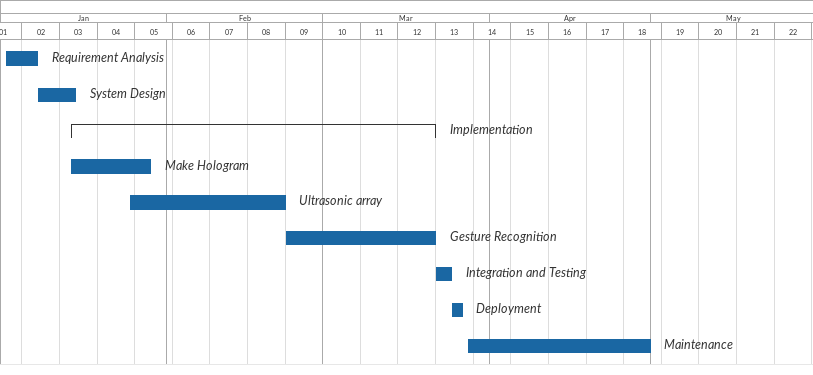
\includegraphics[scale=.6]{images/work_plan.png}
        \caption{Work Plan}
        \end{center}
        \end{figure}
 \section{Budget}
\chapter{Conclusion}

An intrusion detection system (IDS) \cite{nist} is a device or software application that monitors network and/or system activities for malicious activities or policy violations and produces reports to a Management Station.


Donald Ervin Knuth \cite{knuth} is a computer scientist and Professor Emeritus at Stanford University. He is the author of the seminal multi-volume work The Art of Computer Programming. Knuth has been called the "father" of the analysis of algorithms


\begin{thebibliography}{1}
\bibitem{nist} K. Scarfone and P. Mell, ``Guide to intrusion detection and prevention systems
(idps),'' \textit{NIST Special Publication}, vol. 800, no. 2007, p. 94, 2007.
\bibitem{knuth} Wikipedia, ``Donald knuth.'' \url{http://en.wikipedia.org/wiki/Donald_Knuth}.


\end{thebibliography}
\end{document}
